\chapter{Preliminary results}
\label{sec:preliminary}
\section{Monocular depth perception}
\label{sec:prelim_monocular}
The goal of this research is to use \ac{SSL} to improve obstacle avoidance on \acp{UAV}.
\ac{SSL} will be used for depth estimation as the need to use vision to sense the environment sets \acp{UAV} apart from other vehicles.
The first question to be asked is whether \ac{SSL}-based depth estimation can actually be used on a \ac{UAV}.
At first sight this may seem obvious: why would it not work on a \ac{UAV}?
However, results indicate that this might not be as simple as it appears.

\begin{figure}
\centering
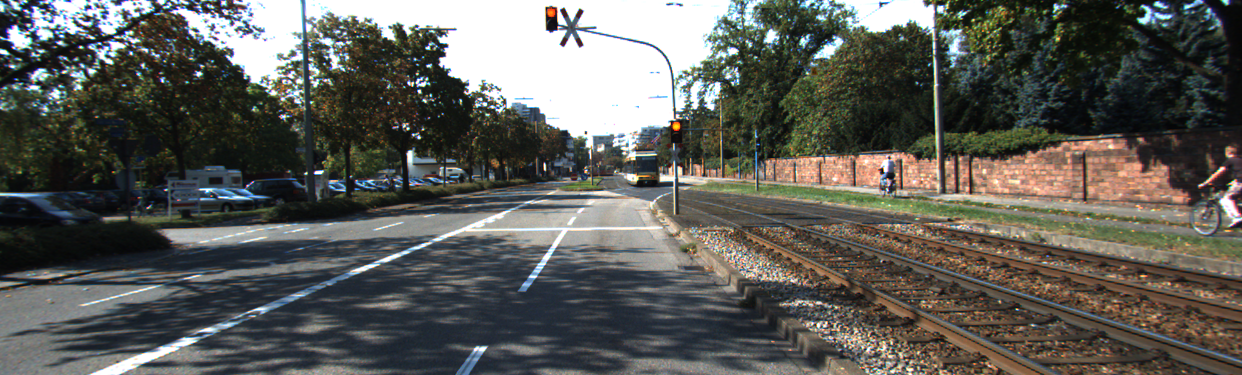
\includegraphics[width=0.45\textwidth]{monodepth.png}
~
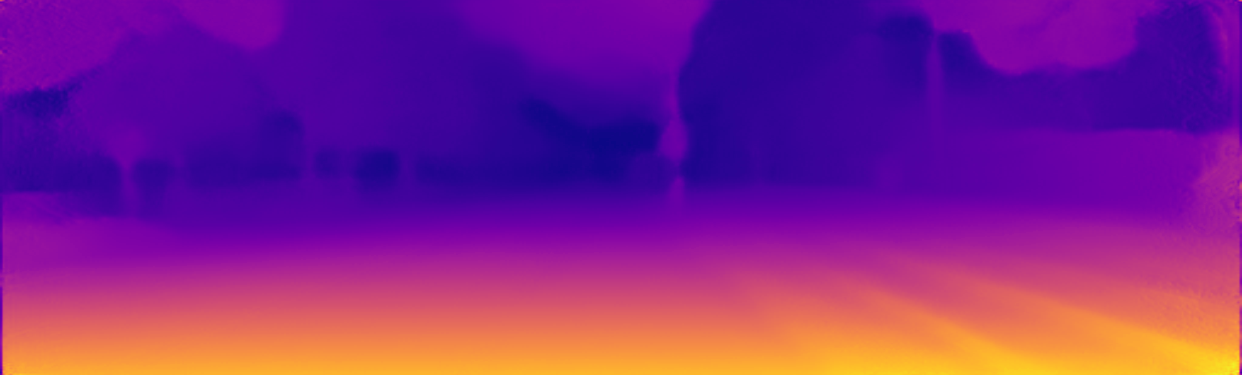
\includegraphics[width=0.45\textwidth]{monodepth_disp.png}
\caption{Monocular depth estimation with \emph{MonoDepth} \cite{Godard2017}.}
\label{fig:monodepth_kitti}
\end{figure}

\begin{figure}
\centering
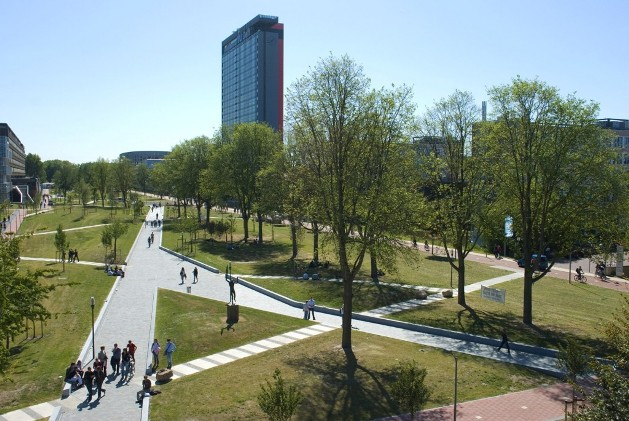
\includegraphics[width=0.45\textwidth]{monodepth_tu.jpg}
~
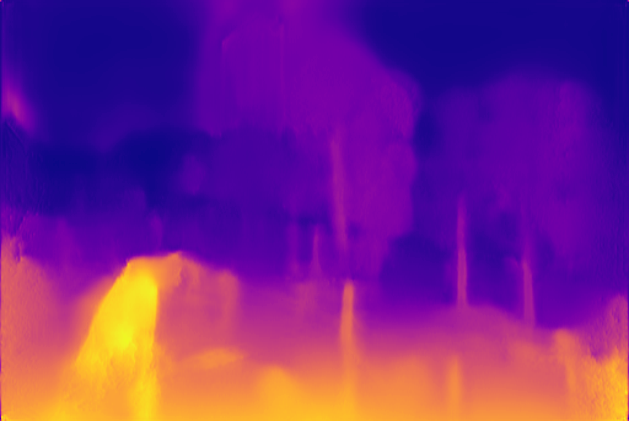
\includegraphics[width=0.45\textwidth]{monodepth_tu_disp.png}
\caption{The MonoDepth network does not transfer well to different viewpoints. The road on the left is seen as a nearby obstacle. The high-rise building of EWI appears closer than the trees in front of it.}
\label{fig:monodepth_tu}
\end{figure}

This chapter presents experiments performed on the \emph{MonoDepth} network \cite{Godard2017}.
MonoDepth is a Self-Supervised monocular depth estimation network that is trained on the KITTI stereo vision dataset.
The network predicts disparities such that these minimize a reconstruction error between two images of a stereo pair.
On images in the KITTI dataset the network performs quite well (\autoref{fig:monodepth_kitti}).
However, when the network is used on images taken from a different viewpoint (\autoref{fig:monodepth_tu}), the accuracy of the depth map quickly degrades.

Clearly, a network trained on a dataset of automotive images cannot be transferred directly to a \ac{UAV}.
Most likely it is possible to get MonoDepth to work on a \ac{UAV} by training it on a suitable dataset.
However, that does not explain why the network trained on KITTI fails.
The results on KITTI images show that the network \emph{can} estimate depth, but apparently it does so using image features that do not work on \acp{UAV}.
To guarantee correct behavior it is important to know what these features are and under what circumstances they are learned.

While there is a large and increasing number of articles on monocular depth perception, there is not a single paper that analyses what these networks actually learn.
This experiment is a first step towards an \emph{understanding} of monocular depth perception as learned by neural networks.
The goals of this experiment are:
\begin{itemize}
\item Provide insight into monocular vision. While useful for \acp{UAV}, this insight will also be extremely valuable for automotive applications. With an understanding of the inner workings of monocular depth perception, it becomes easier to predict its behavior and to make guarantees about its correctness.
\item Provide insight into the use of monocular vision on \acp{UAV}. The results should explain why the network trained on KITTI does not transfer well. The same experiments can then be performed on a network trained on a \ac{UAV} dataset, and the differences can be compared.
\item The features learned by MonoDepth might be replicated using simpler, lightweight algorithms. This would enable the use of monocular vision on embedded hardware and tiny \acp{UAV}, perhaps even the DelFly.
\end{itemize}

The problem with neural networks like MonoDepth is that they are black boxes.
It is difficult to analyze what is going on inside them.
In that aspect there is some overlap with human depth perception, which is also difficult to take apart piece-by-piece.
For neural networks there are techniques to visualize the functions of individual neurons, but this is a very low-level form of analysis.
Instead, the experiments presented here will analyze the behavior of the entire network using the time-tested scientific method: coming up with \emph{hypotheses} on how the network could estimate depth, then designing experiments that \emph{test} whether these hypotheses are true.

So what would be a good hypothesis on the inner workings of MonoDepth?
The experiments performed in this chapter test the following points:
\begin{itemize}
\item MonoDepth assumes there is a flat ground in front of the vehicle.
\item MonoDepth uses color to detect the sky.
\item MonoDepth estimates the distance towards obstacles using one or more of the following features:
\begin{itemize}
\item Apparent size of known obstacles.
\item Vertical position in the image.
\end{itemize}
\end{itemize}
MonoDepth is trained on the KITTI dataset, which contains images taken from a forward-facing camera on a car.
The camera has a fixed attitude and height and in the majority of the images there is a free section of road in front of the car.
Rather than detecting the road, MonoDepth can just assume it is there as this will be true for nearly all images in the training set.
It is hypothesized that MonoDepth assumes the presence of a flat ground rather than detecting it.
The ground's depth estimate will be `overwritten' by any obstacles it detects.

The upper half of the image consists of sky and obstacles.
The sky seems easy to detect using its color or brightness and would result in a large number of correct pixels; it is therefore assumed that MonoDepth does just that, possibly combined with a prior expectation of seeing the sky in the upper half of the image.

With the ground and sky detected, the rest of the depth map consists of obstacles.
Following the list of appearance cues in \autoref{sec:appearance}, likely candidates for depth estimation towards obstacles are their apparent size and vertical position as both seem relatively easy to measure, although the former also requires knowledge about the true size of various types of obstacles.

\medskip

\begin{figure}
\centering
\begin{subfigure}[t]{0.45\textwidth}

\includegraphics[width=\textwidth]{monodepth_horizon_white.png}\\
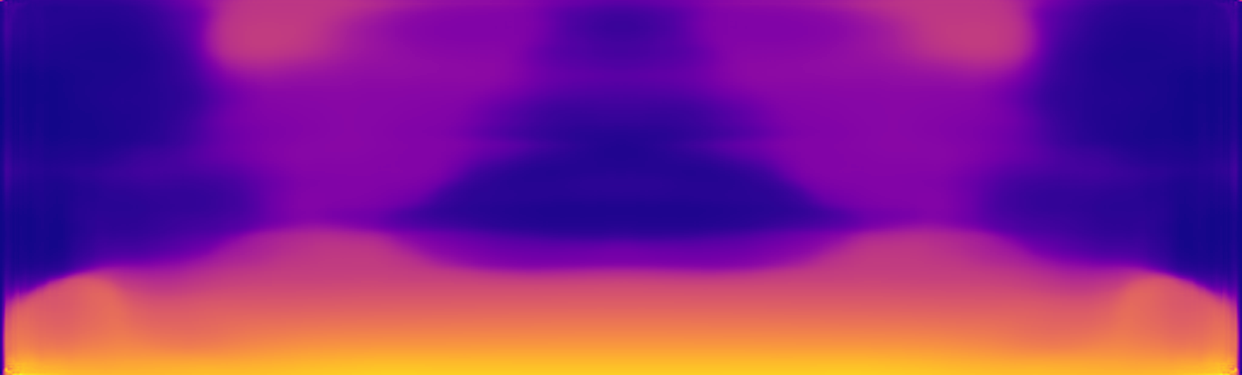
\includegraphics[width=\textwidth]{monodepth_horizon_white_disp.png}
\caption{MonoDepth's response to a completely white input image. Although there is a hint of a ground surface, the depth map (especially the top half) contains a lot of garbage.}
\end{subfigure}
~
\begin{subfigure}[t]{0.45\textwidth}
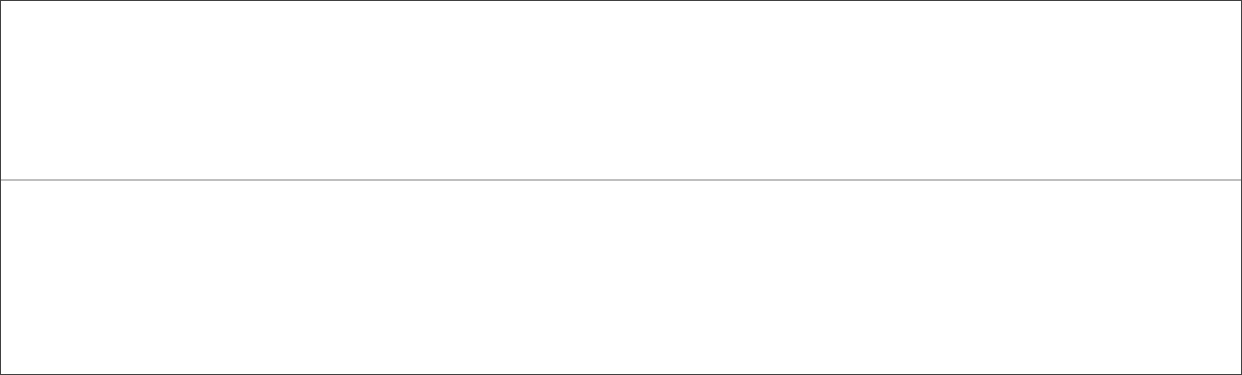
\includegraphics[width=\textwidth]{monodepth_horizon_line.png}\\
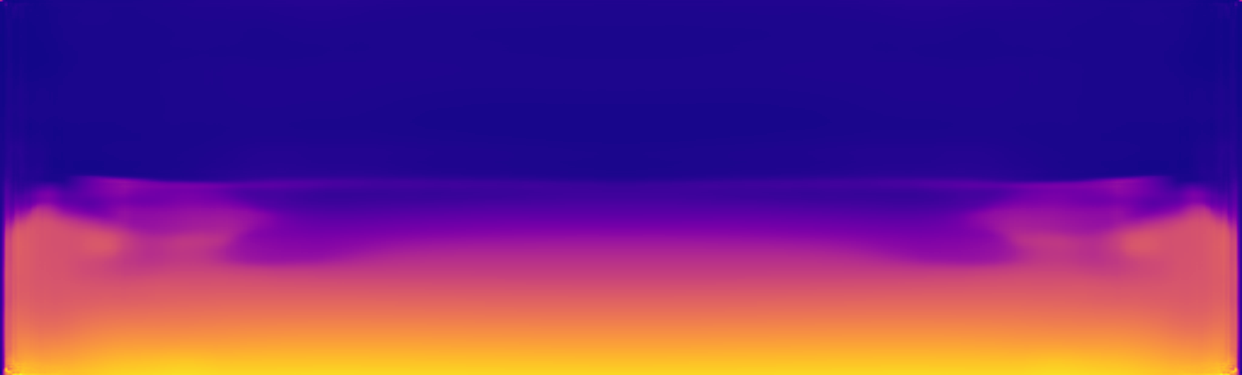
\includegraphics[width=\textwidth]{monodepth_horizon_line_disp.png}
\caption{Addition of a single thin line is enough to make MonoDepth detect a floor and sky, or at least assume they are there.}
\end{subfigure}
\caption{MonoDepth has strong prior expectations about the presence of a flat ground in the lower half of the image and sky in the upper half. (Outlines added for visibility, these are not part of the input images.)}
\label{fig:monodepth_horizon}
\end{figure}

If MonoDepth indeed assumes the presence of a flat ground, it should be possible to make it `see' a ground surface even if it isn't actually there.
This is attempted in \autoref{fig:monodepth_horizon}.
First, MonoDepth is presented with a completely blank input image to see if it will guess the presence of ground and sky.
This is not entirely the case.
However, when a thin horizon line is added to the image, MonoDepth is suddenly able to detect a floor and sky.
Since the input image contains no features other than a single line, these can only come from MonoDepth's prior expectations.

\begin{figure}
\centering
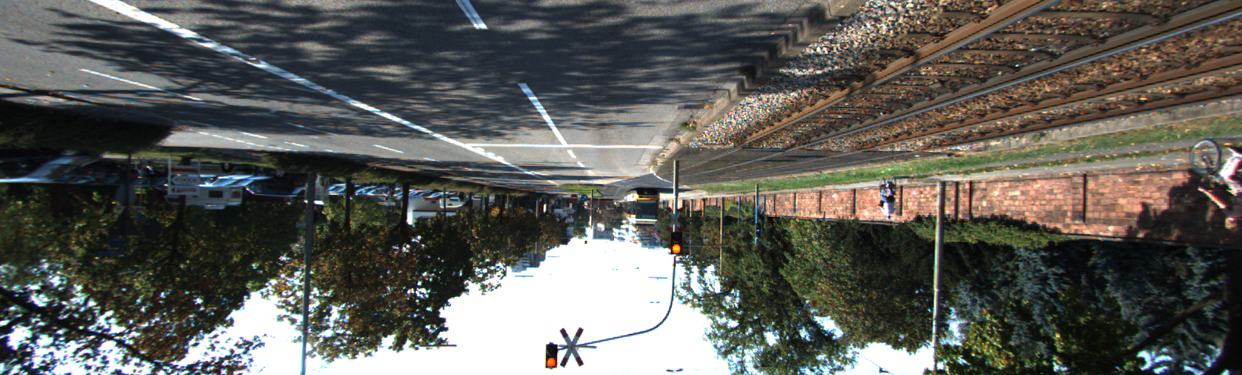
\includegraphics[width=0.45\textwidth]{monodepth_flip.png}\\
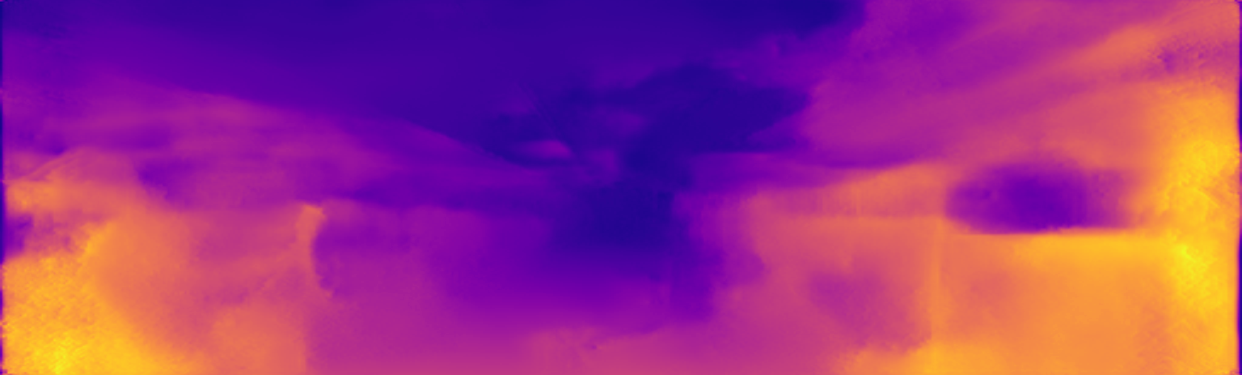
\includegraphics[width=0.45\textwidth]{monodepth_flip_disp.png}
\caption{When the image is flipped vertically, the trees and sky in the lower half of the image are assumed to be closer than the road in the upper half. If MonoDepth did not have prior expectations about a flat ground, the disparity map would also have flipped vertically.}
\label{fig:monodepth_flip}
\end{figure}

This prior expectation can also be demonstrated on real photographs, as shown in \autoref{fig:monodepth_flip}.
In this figure, a vertically flipped image from the KITTI dataset is presented to MonoDepth.
If MonoDepth would not assign a high prior probability to the presence and location of the ground and sky, the resulting depth map would also be a flipped version of the original depth map.
This is, however, not the case.
Instead, the resulting depth map still assumes that the lower half of the image is closer than the upper half, confirming the presence of this bias in the estimation.

\begin{figure}
\centering
\begin{subfigure}[t]{0.3\textwidth}

\includegraphics[width=\textwidth]{monodepth_horizon_line_lower.png}\\
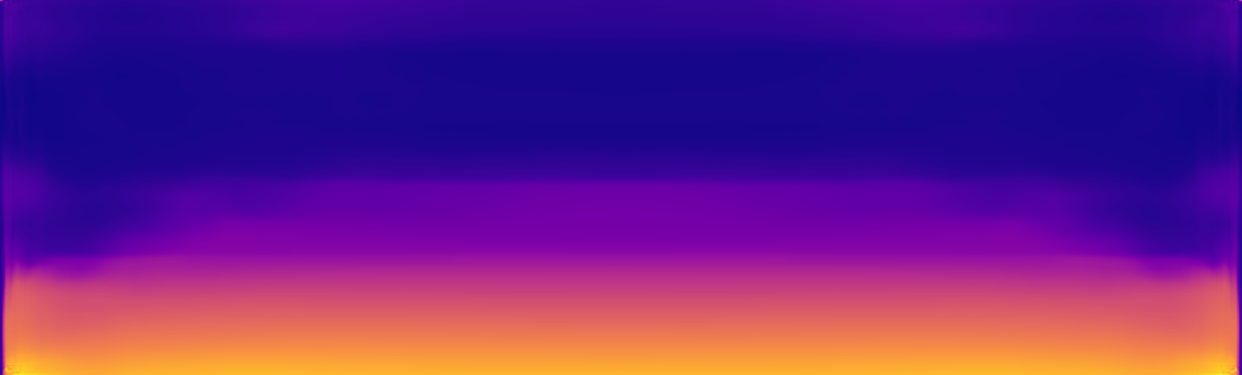
\includegraphics[width=\textwidth]{monodepth_horizon_line_lower_disp.png}
\caption{Lower horizon line.}
\end{subfigure}
~
\begin{subfigure}[t]{0.3\textwidth}
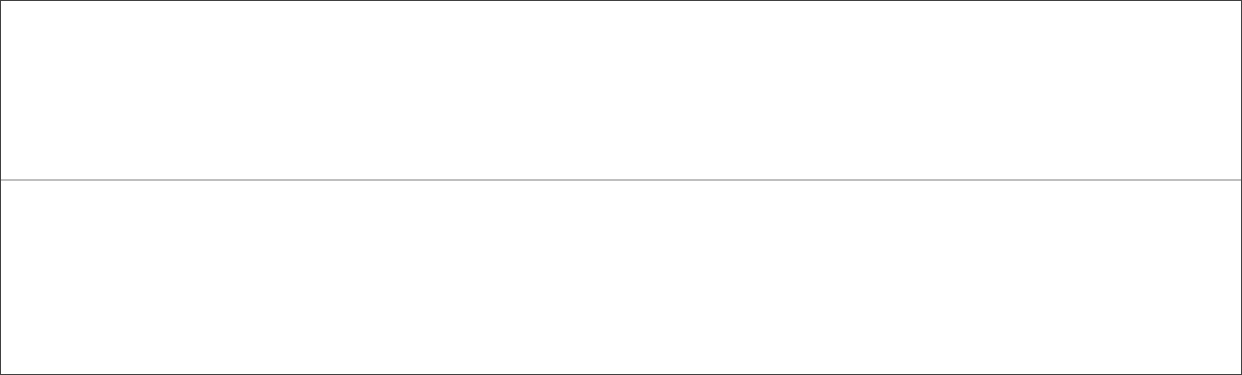
\includegraphics[width=\textwidth]{monodepth_horizon_line.png}\\
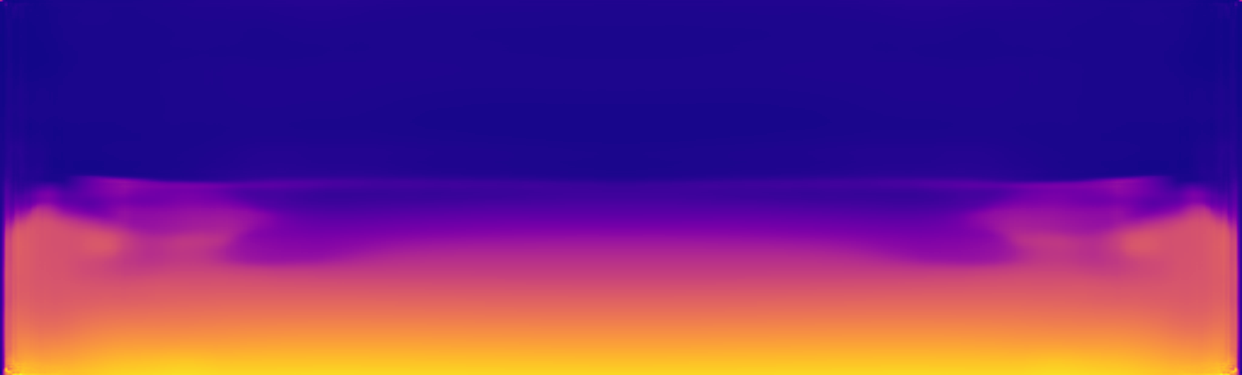
\includegraphics[width=\textwidth]{monodepth_horizon_line_disp.png}
\caption{The original horizon line, aligned with the horizon in the KITTI images.}
\end{subfigure}
~
\begin{subfigure}[t]{0.3\textwidth}

\includegraphics[width=\textwidth]{monodepth_horizon_line_higher.png}\\
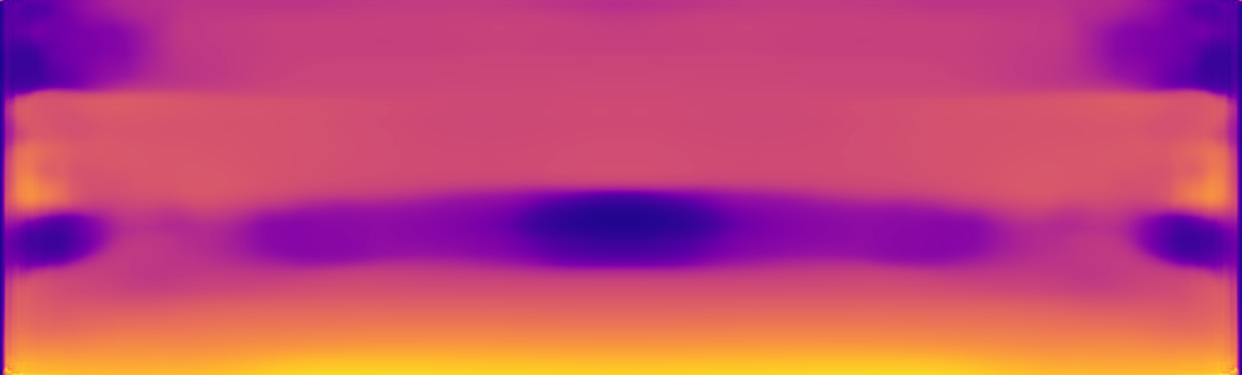
\includegraphics[width=\textwidth]{monodepth_horizon_line_higher_disp.png}
\caption{Higher horizon line.}
\end{subfigure}

\begin{subfigure}[t]{0.3\textwidth}
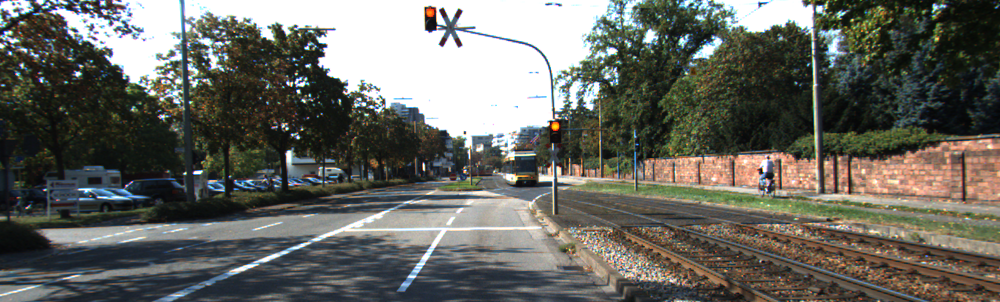
\includegraphics[width=\textwidth]{monodepth_horizon_crop_high.png}\\
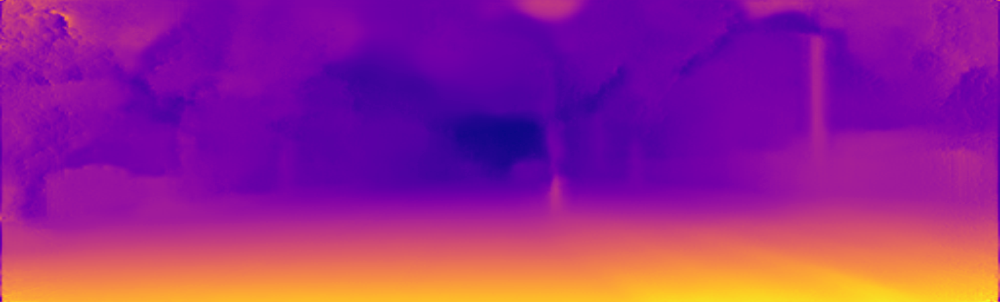
\includegraphics[width=\textwidth]{monodepth_horizon_crop_high_disp.png}
\caption{Lower horizon line.}
\end{subfigure}
~
\begin{subfigure}[t]{0.3\textwidth}
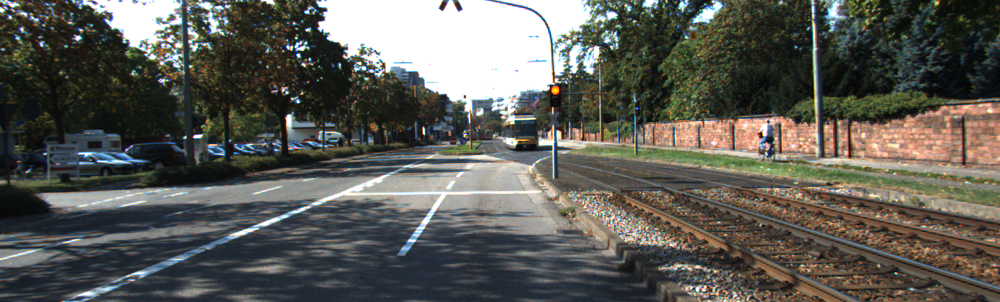
\includegraphics[width=\textwidth]{monodepth_horizon_crop_center.png}\\
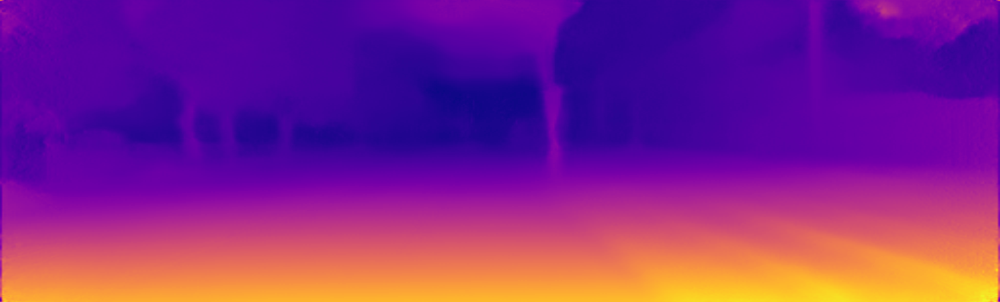
\includegraphics[width=\textwidth]{monodepth_horizon_crop_center_disp.png}
\caption{Original horizon line.}
\end{subfigure}
~
\begin{subfigure}[t]{0.3\textwidth}
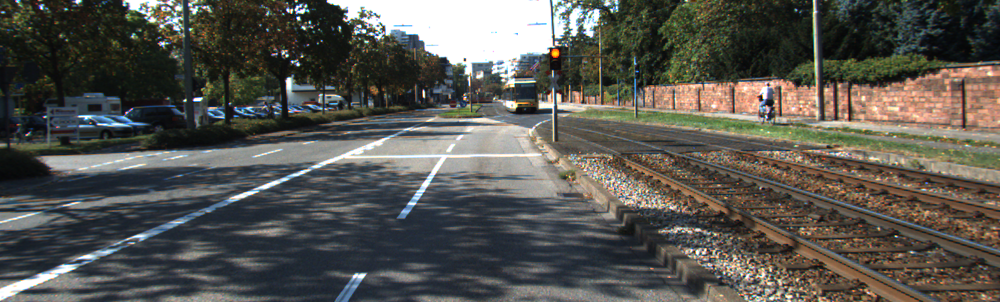
\includegraphics[width=\textwidth]{monodepth_horizon_crop_low.png}\\
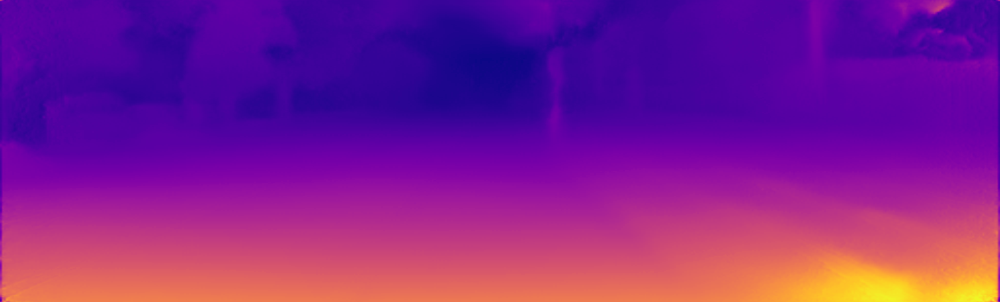
\includegraphics[width=\textwidth]{monodepth_horizon_crop_low_disp.png}
\caption{Higher horizon line.}
\end{subfigure}
\caption{\emph{a-c}: The vertical position of the horizon line does not change the ground plane. While it has some influence on the depth map, the ground plane still seems to end at the same height in the image.
\emph{d-f}: In real images, the extent of the ground plane matches the position of the horizon. This suggests that MonoDepth has a mechanism to detect the horizon that is not triggered in images \emph{a-c}; it is not yet understood how this works.}
\label{fig:monodepth_pitch}
\end{figure}

It appears that MonoDepth indeed assumes the presence of a flat ground in the lower half of the image, but does it assume a fixed depth map for the ground or does it detect the horizon in the input image?
The latter would allow the network to correct changes in the pitch of the camera.
To test this, the network is first presented with artificial images based on \autoref{fig:monodepth_horizon}, but with the horizon line shifted to different positions.
The result is shown in \autoref{fig:monodepth_pitch} a-c.
In these artificial images it seems that MonoDepth does not use the position of the line for the ground plane, although it does have some influence on the depth map.
This is also tested on real images by cropping different regions from one of the KITTI images, see \autoref{fig:monodepth_pitch} d-f.
The result is different; now the ground plane in the depth maps ends at the horizon in the input image.
Apparently MonoDepth does estimate the position of the horizon.
At the time of writing it is not yet clear how this works.
Note that MonoDepth's correction to the pitch is not perfect: the depth towards obstacles appears to have changed, especially in \autoref{fig:monodepth_pitch}~d.

\begin{figure}
\centering
\begin{subfigure}[t]{0.45\textwidth}
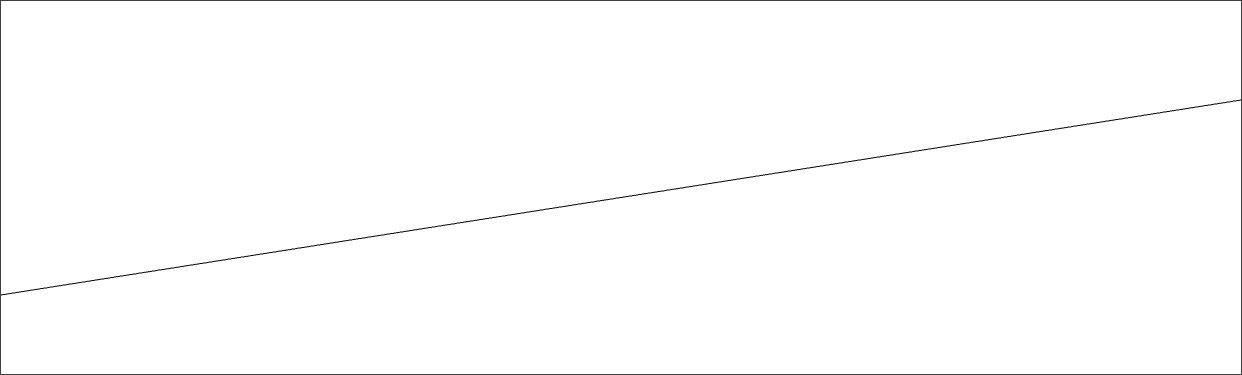
\includegraphics[width=\textwidth]{monodepth_horizon_angled.png}
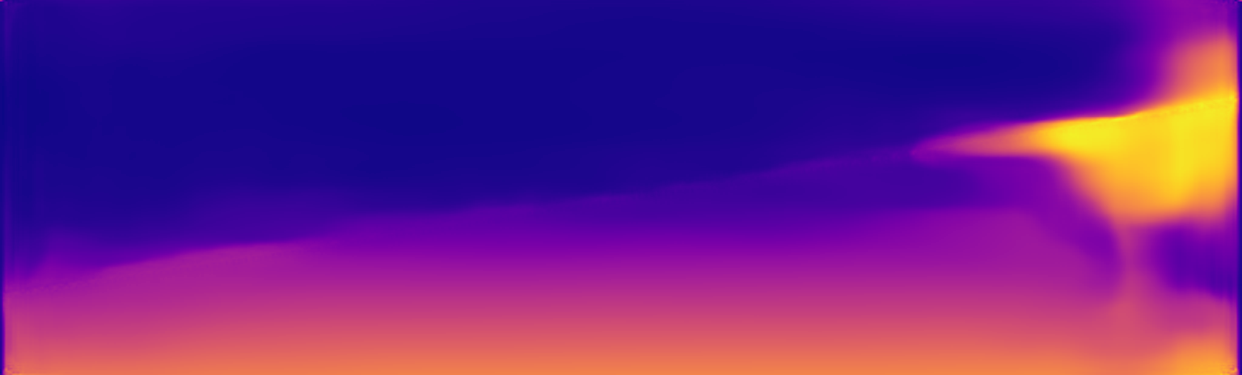
\includegraphics[width=\textwidth]{monodepth_horizon_angled_disp.png}
\caption{When the artificial horizon line is tilted, the ground surface remains flat in the depth map. There are some artefacts where the line is above the assumed horizon.}
\end{subfigure}
~
\begin{subfigure}[t]{0.45\textwidth}
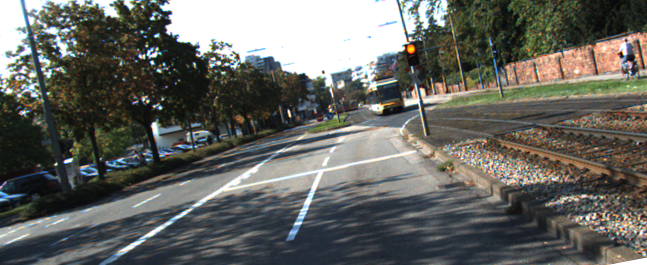
\includegraphics[width=\textwidth]{monodepth_angle.png}\\
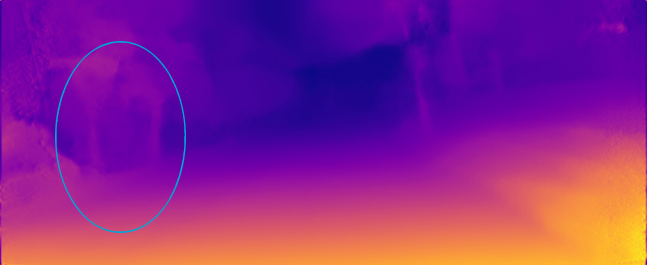
\includegraphics[width=\textwidth]{monodepth_angle_disp.png}
\caption{Even though the input image is tilted, the road surface appears more-or-less flat in the disparity map. Also notice the trees that are vertical in the disparity map but clearly tilted in the input image.}
\end{subfigure}
\caption{Both in artificial and real images MonoDepth does not appear to detect roll motions and will still assume a flat road surface and vertically oriented obstacles.}
\label{fig:monodepth_roll}
\end{figure}

Does MonoDepth also detect roll angles?
This is tested by rotating the input images, the result is shown in \autoref{fig:monodepth_roll}.
It appears that MonoDepth does not detect the roll angle of the camera: the ground surface still appears flat.
Also note the tree trunks that appear vertical in the depth map even though they are clearly tilted in the input image.
This seems another example of MonoDepth assuming the presence of certain features rather than actually observing them.

\medskip

\begin{figure}
\centering
\begin{subfigure}[t]{0.45\textwidth}
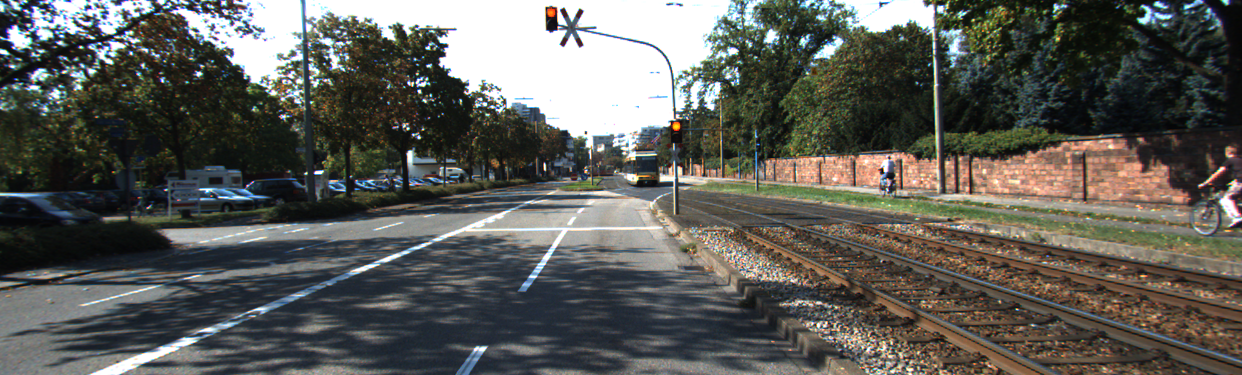
\includegraphics[width=\textwidth]{monodepth.png}\\
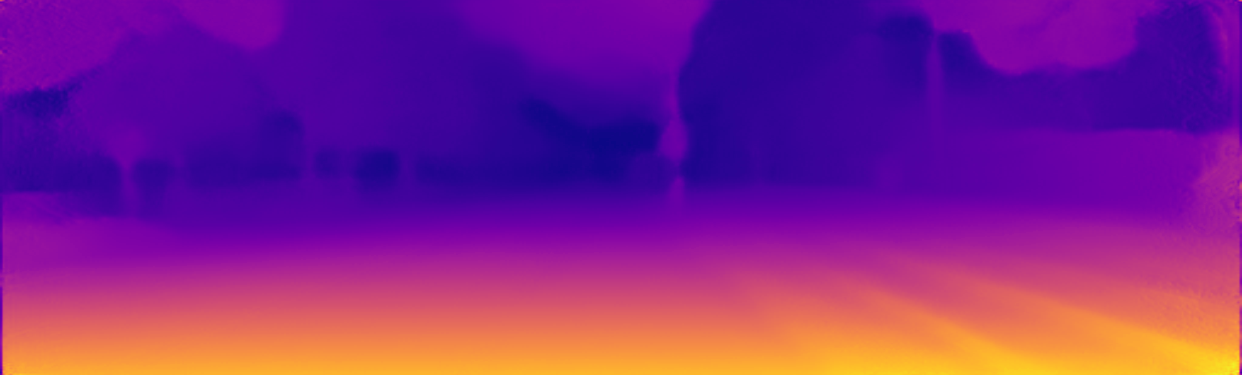
\includegraphics[width=\textwidth]{monodepth_disp.png}
\caption{Original image.}
\end{subfigure}
~
\begin{subfigure}[t]{0.45\textwidth}
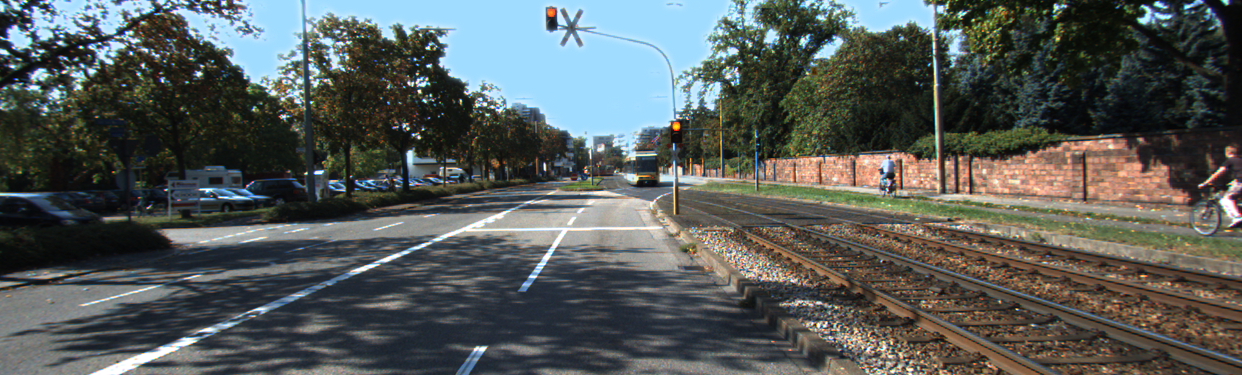
\includegraphics[width=\textwidth]{monodepth_sky_blue.png}\\
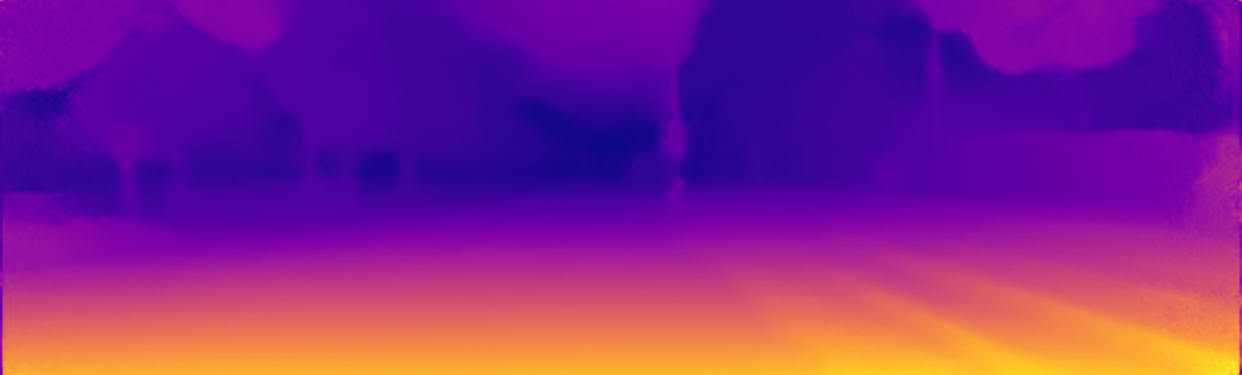
\includegraphics[width=\textwidth]{monodepth_sky_blue_disp.png}
\caption{Blue sky. No difference in the depth map.}
\end{subfigure}

\begin{subfigure}[t]{0.45\textwidth}
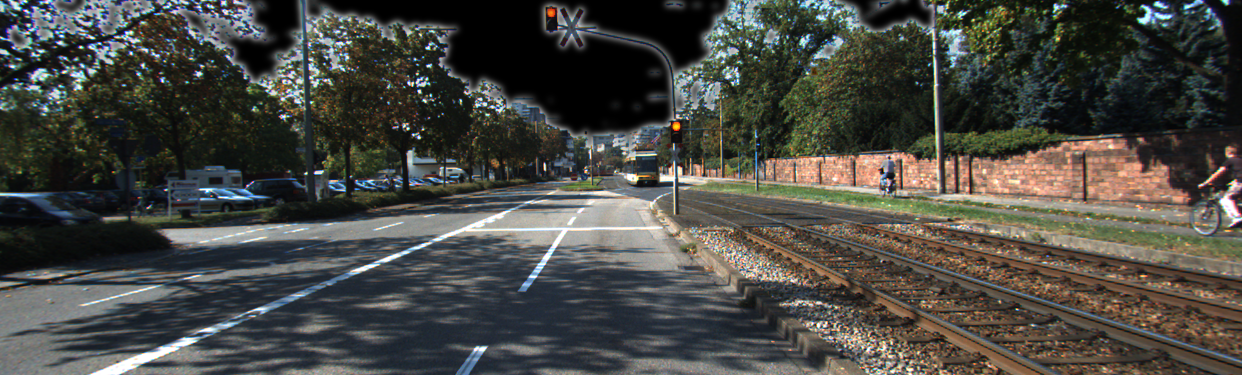
\includegraphics[width=\textwidth]{monodepth_sky_black.png}\\
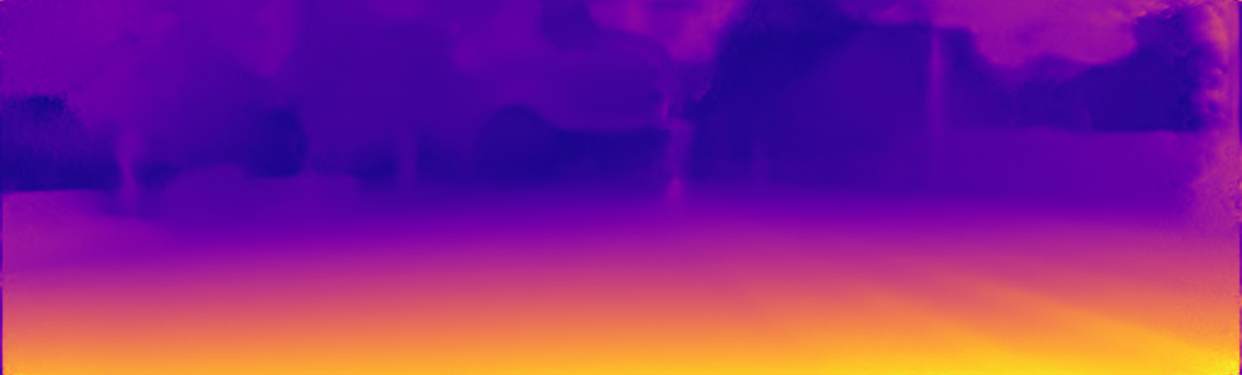
\includegraphics[width=\textwidth]{monodepth_sky_black_disp.png}
\caption{Black sky. The sky appears further away, there are some artifacts around the traffic light.}
\end{subfigure}
~
\begin{subfigure}[t]{0.45\textwidth}
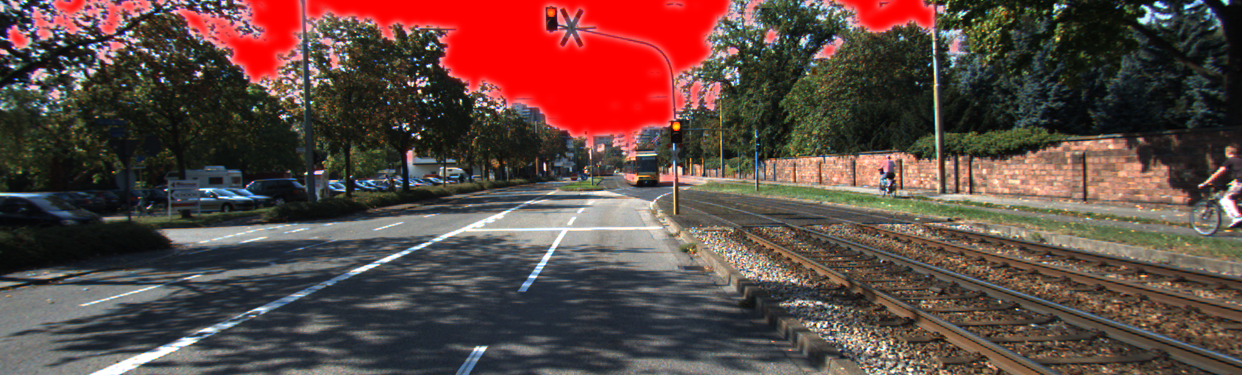
\includegraphics[width=\textwidth]{monodepth_sky_red.png}\\
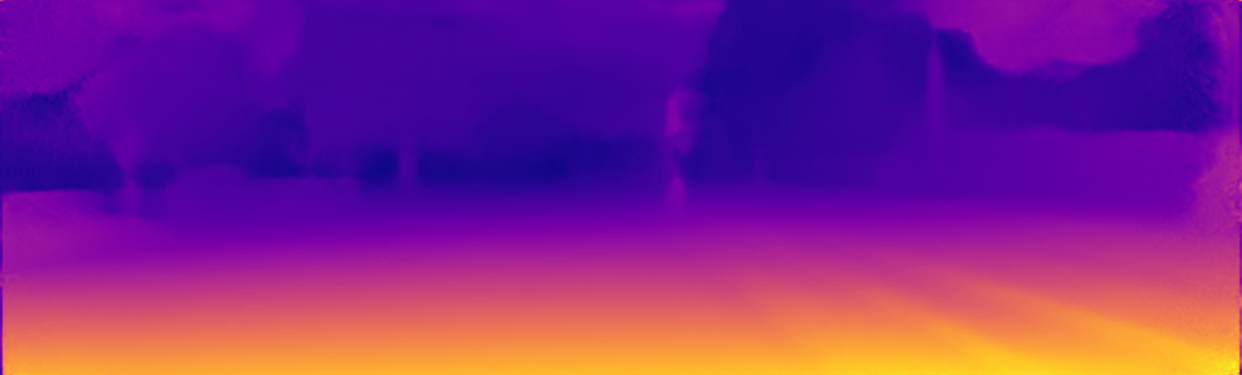
\includegraphics[width=\textwidth]{monodepth_sky_red_disp.png}
\caption{Red sky. The sky appears further away.}
\end{subfigure}
\caption{Sensitivity to sky color. There is no perceivable difference between the depth maps for white and blue sky, colors that naturally occur in the training dataset. There is some difference when the sky is made black or red, but the effect remains relatively small.}
\label{fig:monodepth_skycolor}
\end{figure}

The second hypothesis is that MonoDepth detects the sky using color segmentation.
While this sounds plausible, \autoref{fig:monodepth_kitti} already hints that this is not entirely true: in the depth map the sky appears closer than the trees that occlude it.
\autoref{fig:monodepth_flip} also shows that there is a prior expectation of the position of the sky in the upper half of the image; the sky color in the bottom half of the image does not result in an infinite depth (although its observed depth is further than that of the trees).

In \autoref{fig:monodepth_skycolor} the sky is replaced with different colors.
The figure shows that unnatural colors have some effect on the depth estimate, but do not cause large disturbances such as objects appearing at close distance.
These results show that MonoDepth does not detect the sky using (only) color segmentation.
What mechanism it uses instead remains to be found in further research.

\medskip

\begin{figure}
\centering

\includegraphics[width=0.45\textwidth]{monodepth_road.png}\\
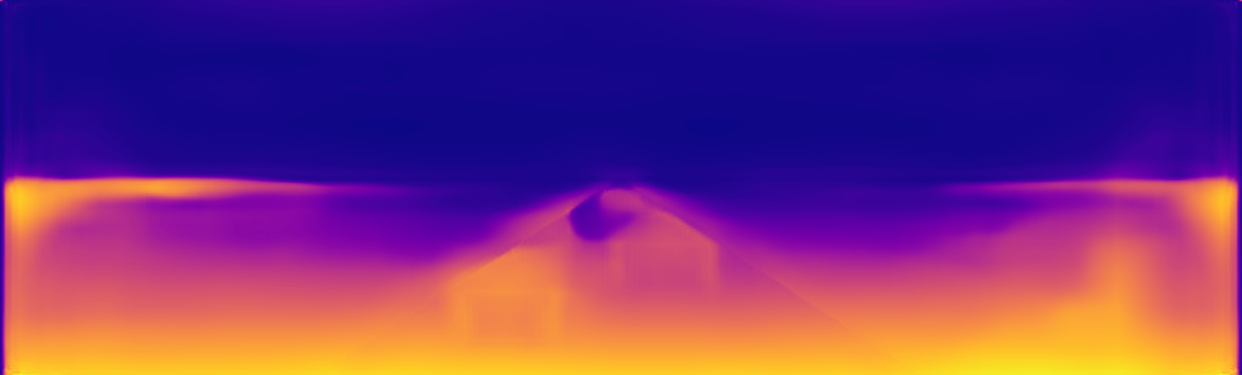
\includegraphics[width=0.45\textwidth]{monodepth_road_disp.png}
\caption{MonoDepth's depth perception can easily be triggered using simple visual features. Notice how the right rectangle appears to be further away than the left, even though they are the same size.}
\label{fig:monodepth_rectangles}
\end{figure}

The final hypothesis on the workings of MonoDepth concerns the depth estimation of obstacles.
Two options appear likely: the obstacle's size is used, or its vertical position in the image.

\autoref{fig:monodepth_rectangles} provides a first clue.
The image shows that MonoDepth's perception of obstacles is easy to trigger: black rectangles are already shown as obstacles in the depth map.
More importantly, however, is how it determined the distance towards the rectangles: the rectangles are the same size in the image but at different vertical positions.
They are placed at different depths, which suggests that the vertical position had a strong influence on this estimate.

\begin{figure}
\centering
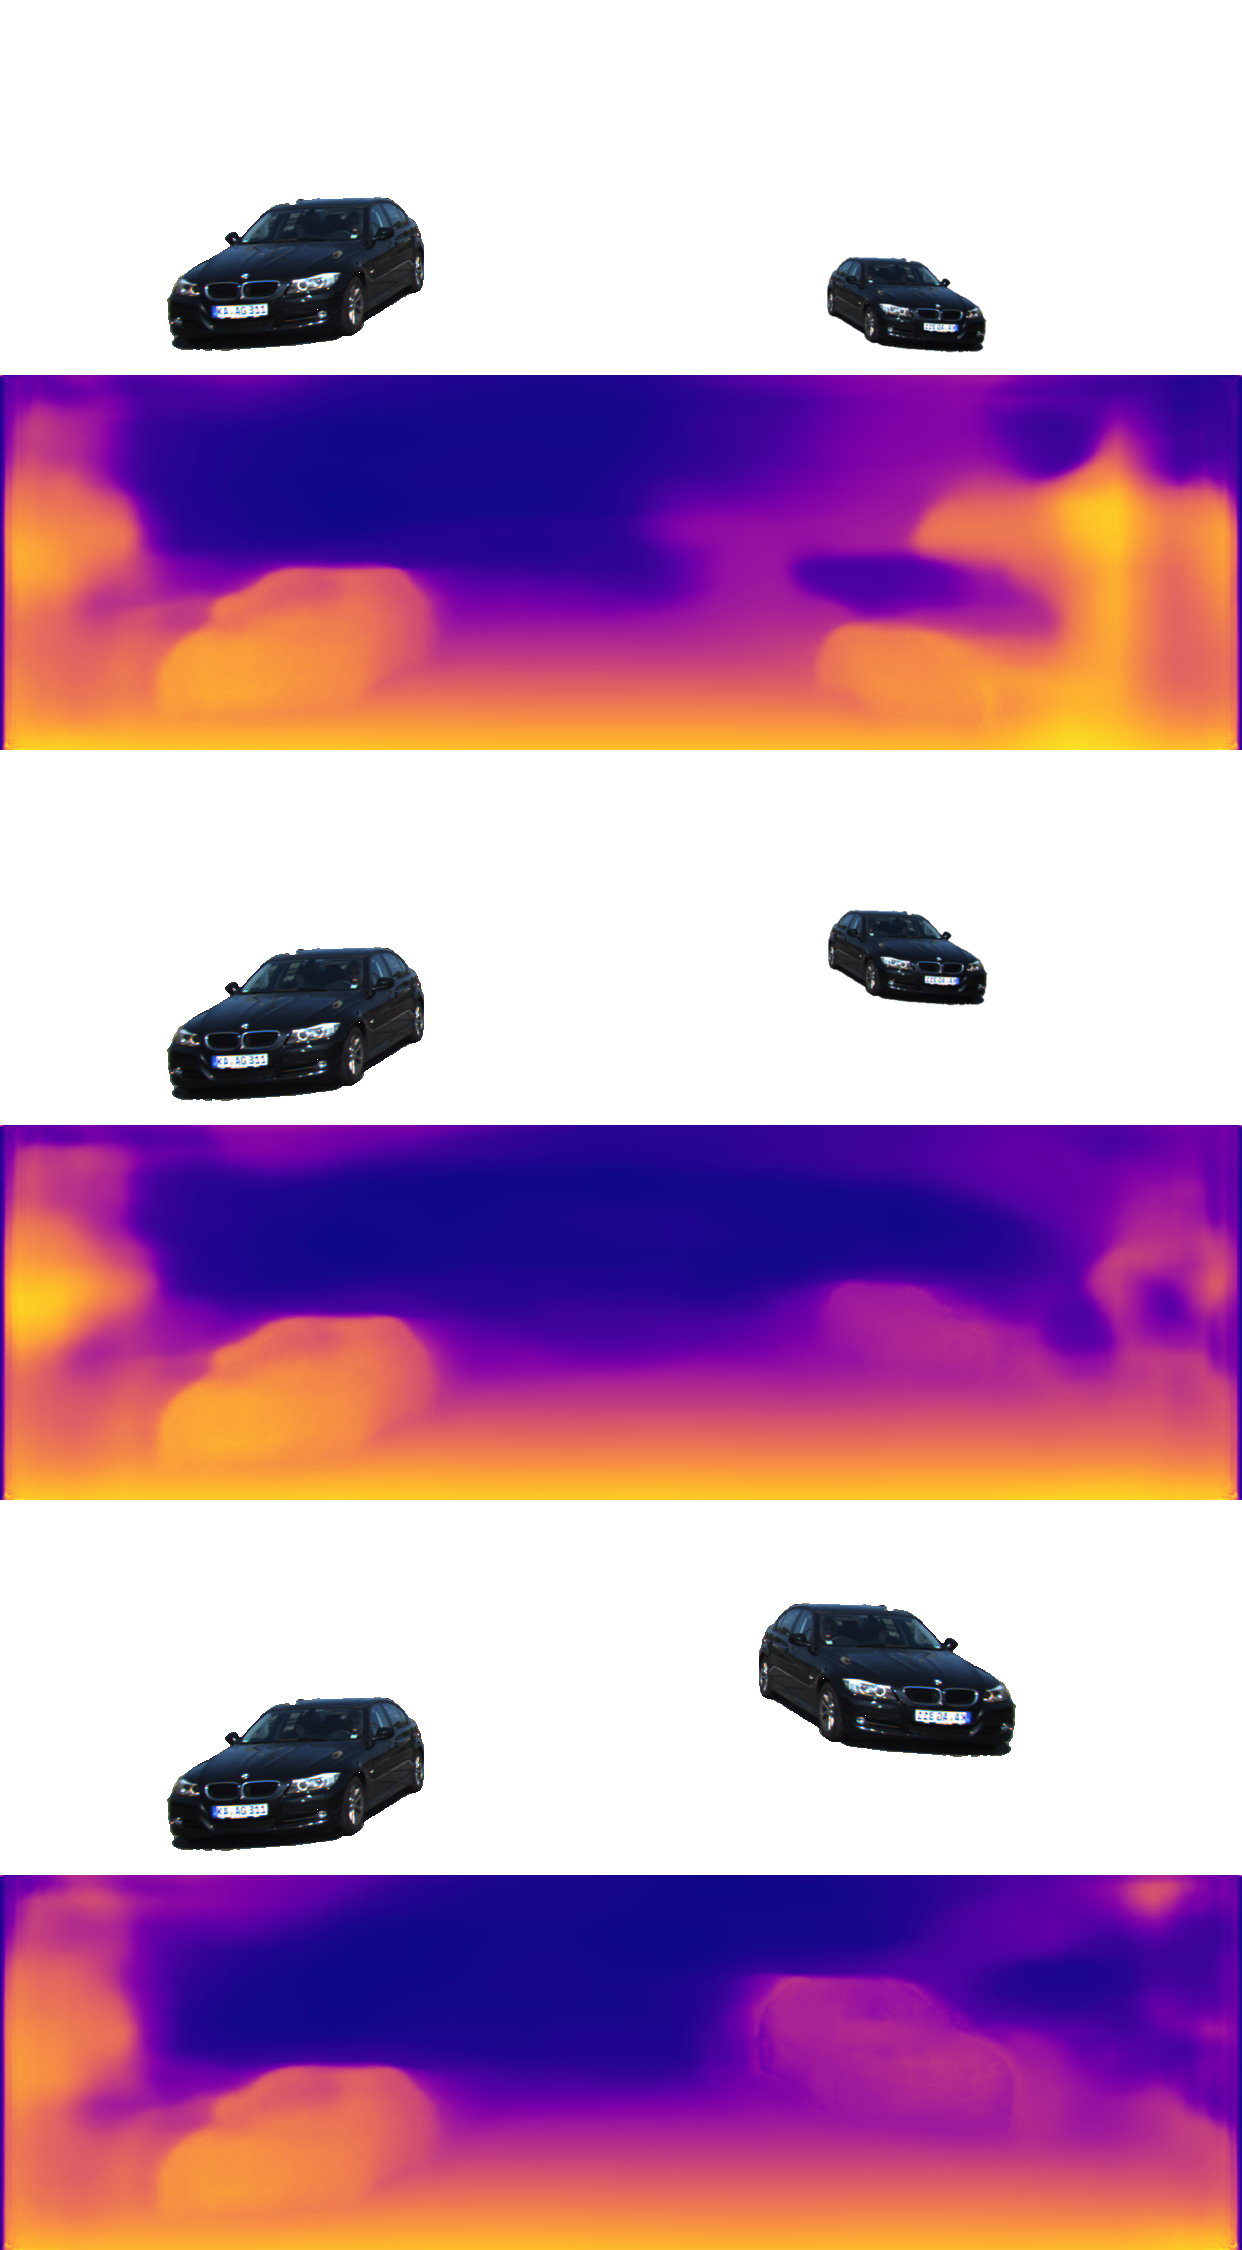
\includegraphics[width=0.45\textwidth]{monodepth_vertical.png}
\caption{MonoDepth's depth estimation depends on the vertical position of objects in the image, not their apparent size.
\emph{Top}: the cars are assigned the same disparity, even though the car on the right has a smaller apparent size.
\emph{Middle}: the right car is smaller and positioned higher in the image (as would be the case in real images), it is correctly estimated to be further away.
\emph{Bottom}: the car on the right has the same apparent size as the one on the left. Still, it is indicated to be further away as its vertical position in the image is higher.}
\label{fig:monodepth_vertical}
\end{figure}

Further evidence towards this conclusion is presented in \autoref{fig:monodepth_vertical}.
In this figure, three scenarios are presented to the network: the real-life scenario in which one car is smaller and higher in the image, one where the car is only smaller, and one where it is only placed at a higher position.
In all cases, the vertical position of the car appears to control the depth estimate.

A final clue can be found back in \autoref{fig:monodepth_pitch}~d where the camera pitch was changed.
When the camera is pitched up, the obstacles move downwards in the image.
In the resulting depth map, the obstacles appear closer.

There are a few possible reasons why the vertical position is used as the main cue for depth.
First of all, it might be easier for a \ac{CNN} to measure the vertical position than the scale of obstacles because the convolution operation is translation-invariant but not scale invariant.
Secondly, since the camera is fixed at a nearly constant height and attitude, distance estimates based on the vertical image position may be more accurate than estimates based on the scale as the latter depend on the real-world dimensions of the obstacle which can contain large variations.

\medskip

What do these results mean for the use of MonoDepth on a \ac{UAV}?
The strong assumption of a flat ground in front of the camera is not compatible with the large pitch and roll angles expected on a \ac{UAV}.
The same holds for the use of vertical image position to estimate the depth towards obstacles: this assumes a constant height above the ground and a constant pitch angle.
In conclusion, MonoDepth trained on the KITTI dataset can not be directly transferred to a \ac{UAV}.
Training on a suitable dataset for \acp{UAV} should reveal whether these problems come from the use of the KITTI dataset for training or whether they are more fundamental.

\medskip

\noindent
\emph{In 2019 a conference paper on this topic was published at the International Conference on Computer Vision:}\nocite{Dijk2019}

\begin{quote}
Tom van Dijk and Guido de Croon.  How Do Neural Networks See Depth in Single Images? In \emph{The IEEE International Conference on Computer Vision (ICCV)}, October 2019. \url{http://openaccess.thecvf.com/content_ICCV_2019/html/van_Dijk_How_Do_Neural_Networks_See_Depth_in_Single_Images_ICCV_2019_paper.html}
\end{quote}